\section{System \"Ubersicht}

\subsection{Komponentendiagramm}

\begin{figure}[H]
  \centering
  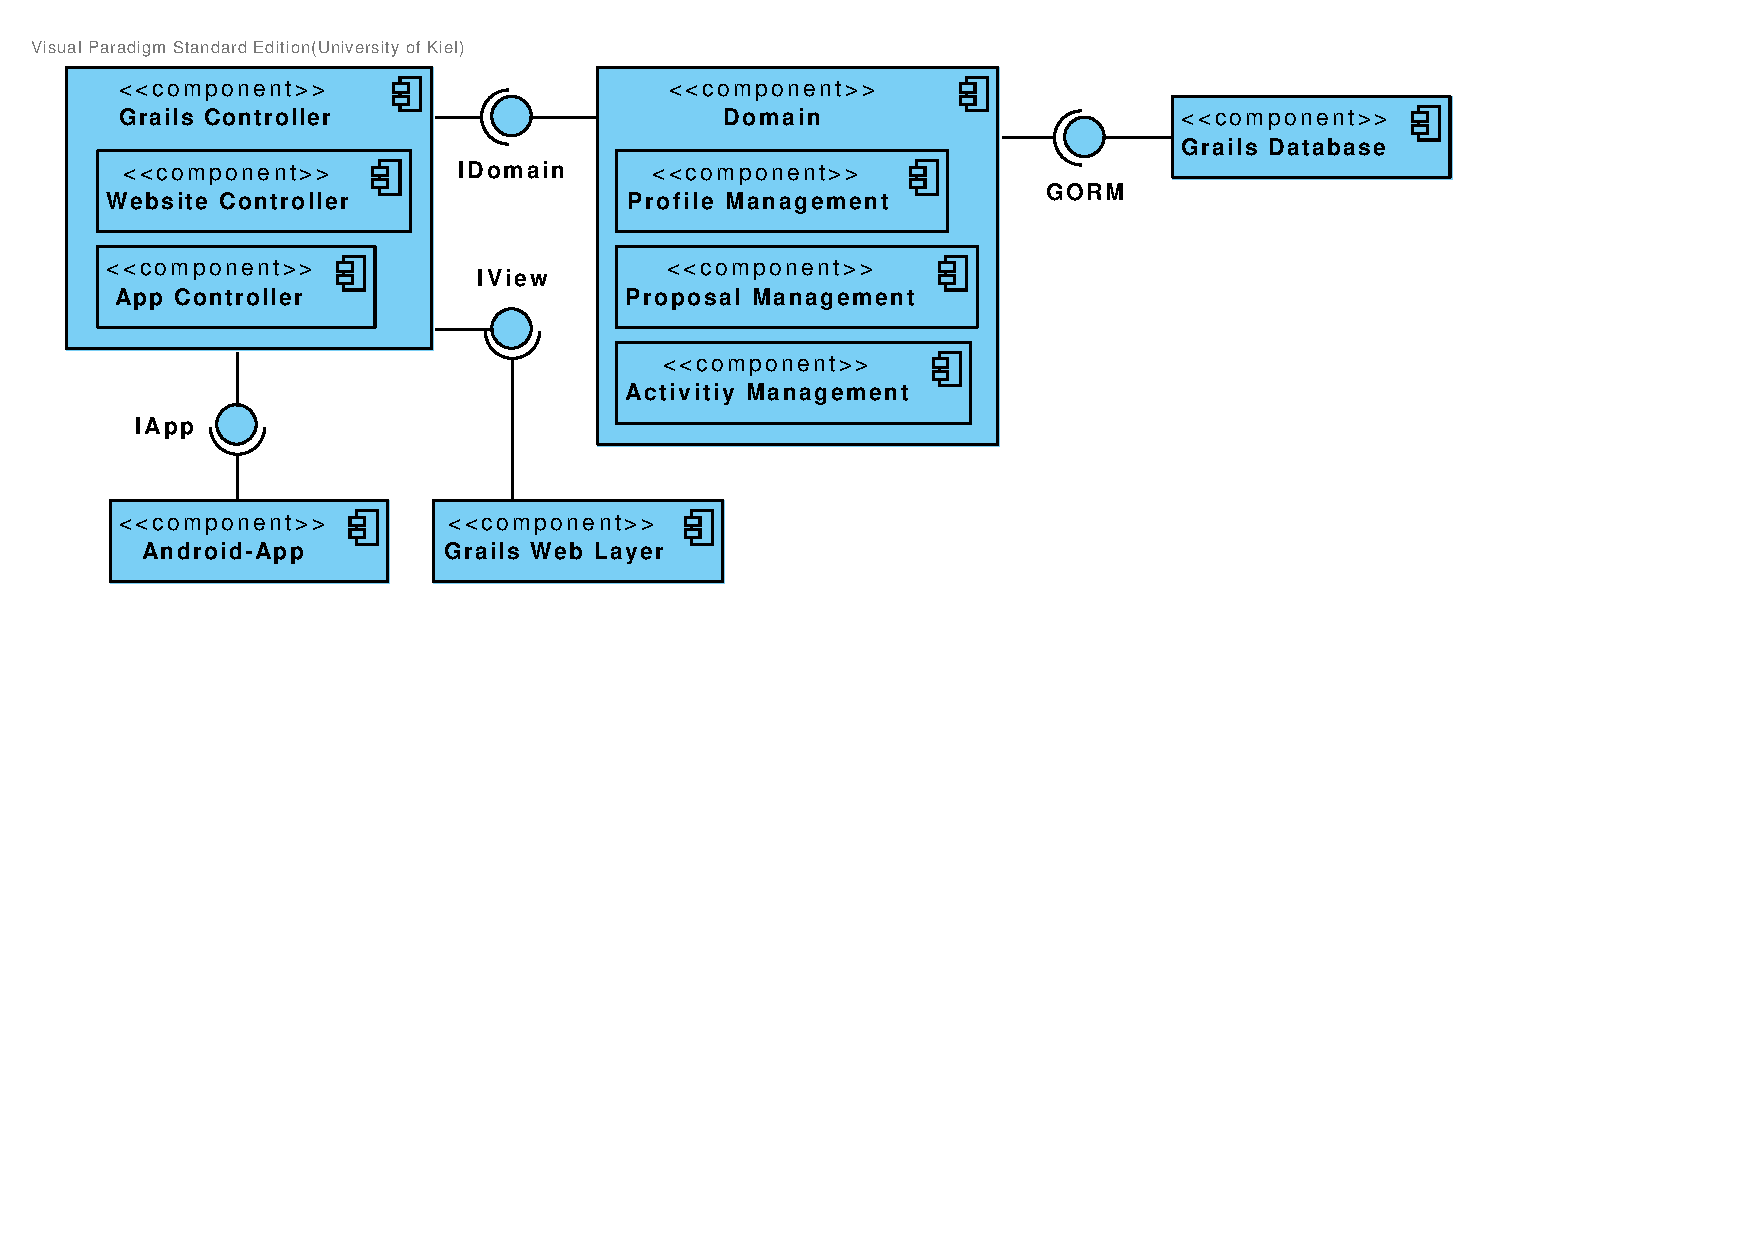
\includegraphics[width=\textwidth, trim=1cm 11cm 4cm 1cm, clip]{gfx/component_diagram}
  \caption{Komponentendiagramm}
\end{figure}

\paragraph{Grails Database} Die Grails Database Komponente ist die zentrale Datenbank, die auf dem Server liegt und s\"amtliche Daten enth\"alt, auf die, \"uber das durch \emph{Grail's Object Relational Mapping} (GORM) bereitgestellte Interface, zugegriffen werden kann.

\paragraph{Domain} Die Domain Komponente ist die Modell
Repr\"asentation der Daten in der Datenbank. Der Zugriff erfolgt
\"uber das IDomain Interface. Die Domain Komponenten ist unterteilt in
die Subkomponenten \emph{Profile Management}, \emph{Proposal
  Management} und \emph{Activity Management}. Das Profile Management
ist zuständig für die Verwaltung der Modellrepräsentation von Team-
und Benutzerprofilen. Das Proposal Managment ist zuständig für die
Verwaltung der Modellrepräsentation von (Aktivitäts-) Vorschlägen. Die
Komponente Activity Management ist zuständig für die Verwaltung der Modellrepräsentation von Aktivitäten.

\paragraph{Grails Web Layer} Die Grails Web Layer Komponente kommuniziert mit dem Grails Controller \"uber das IView Interface und stellt die GSP Dateien zur Verf\"ugung, die das Layout der Website spezifizieren.

\paragraph{Grails Controller} Die Controller Komponente besteht aus den einzelnen Controllern f\"ur Website und Android App und ist zust\"andig f\"ur die Verarbeitung s\"amtlicher Daten und Anfragen, die \"uber die IApp, IDomain und IView Schnittstellen kommuniziert werden.

\paragraph{Android App} Die Android App, dient in erster Linie zur Repr\"asentation der Daten vom Server auf Mobilger\"aten. Sie kommuniziert \"uber das IApp Interface mit dem Controller.

\subsection{Verteilungsdiagramm}

\begin{figure}[H]
  \centering
  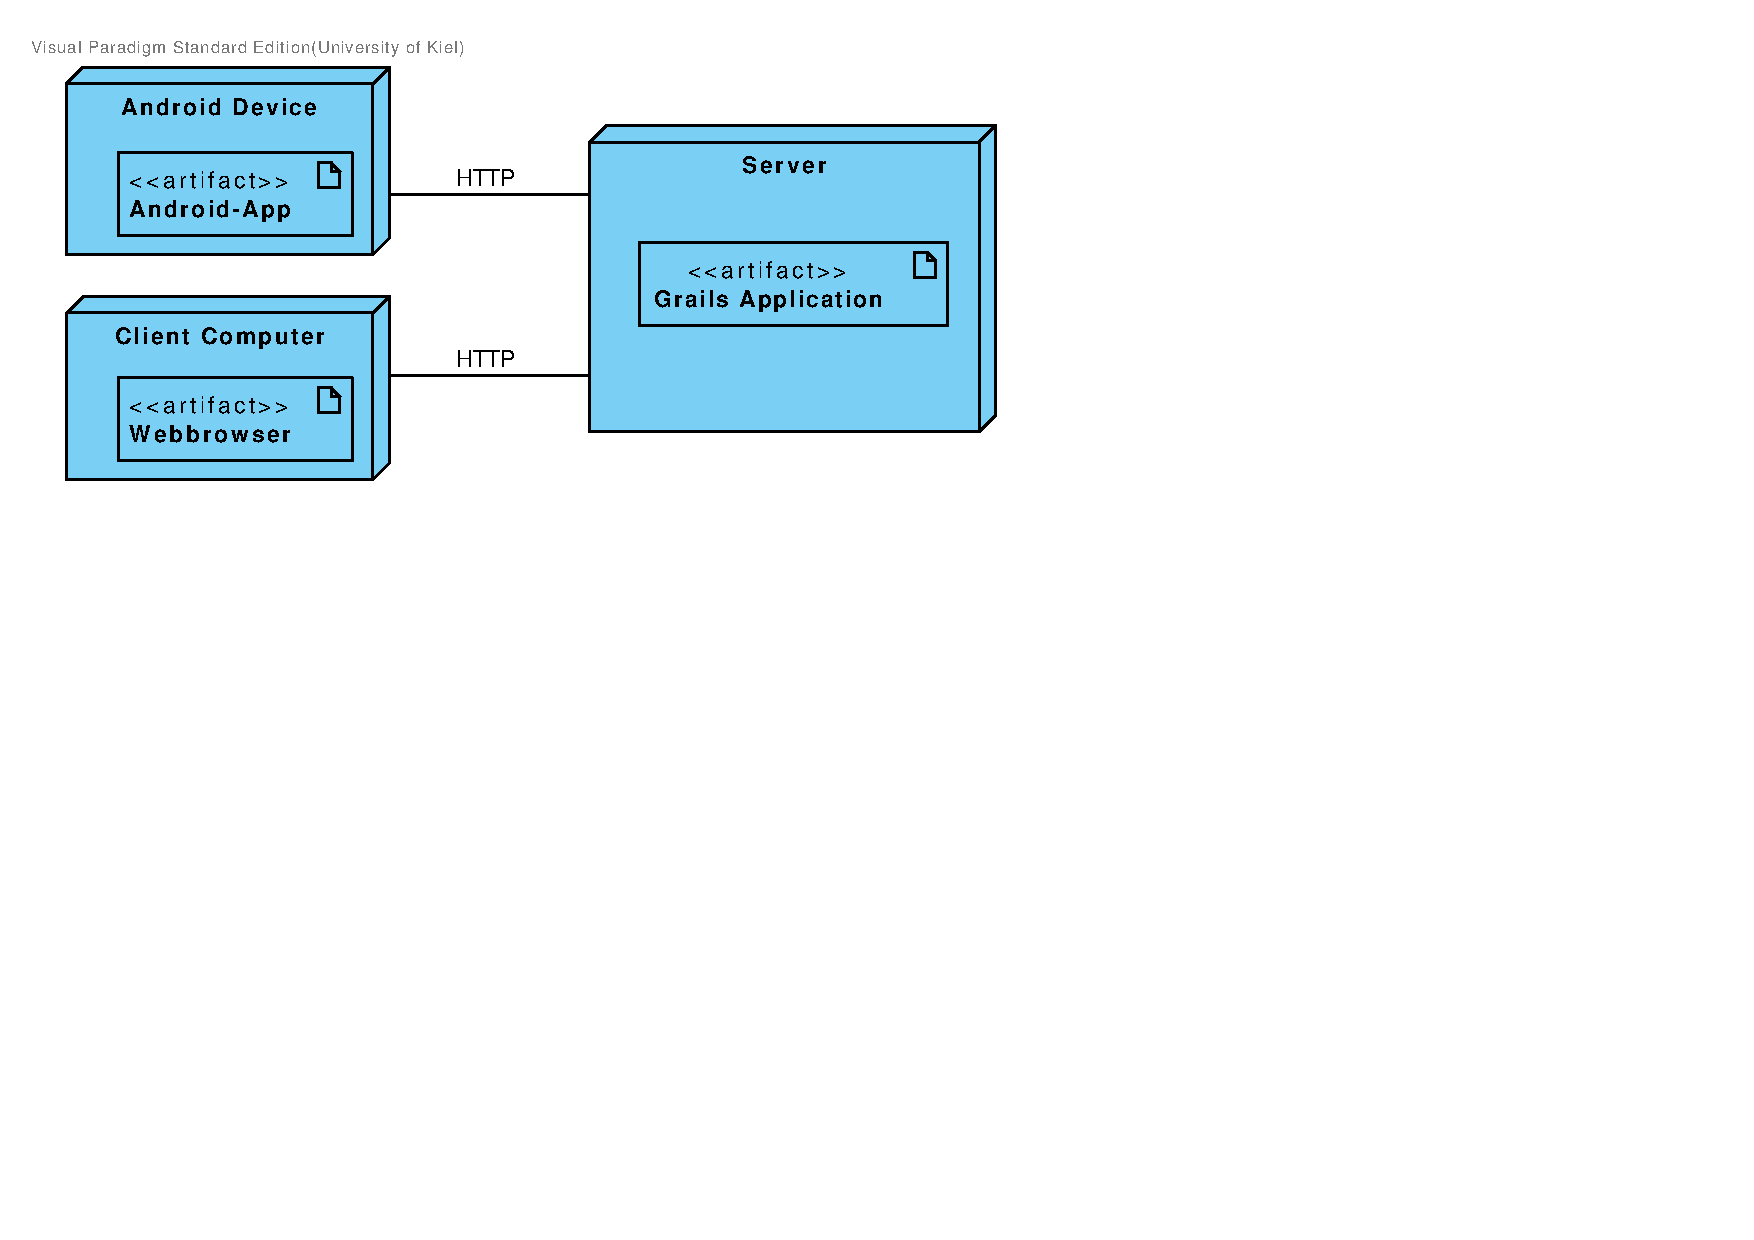
\includegraphics[width=\textwidth, trim=1cm 12cm 12cm 1cm, clip]{gfx/deployment_diagram}
  \caption{Verteilungsdiagramm}
\end{figure}

\paragraph{Client Computer}
Benutzer können mit Hilfe eines Computers über einen Webbrowser auf eine Website zugreifen, welche, nach erfolgreichem einloggen, verschiedene Funktionen zur Aktivitäts- und Profilverwaltung anbietet.Des Weiteren können hier auch anonymisierte Statistiken angezeigt und diese statistischen Daten exportiert werden.

\paragraph{Android Device}
Über ein Android Gerät haben die Benutzer die Möglichkeit an der EnergyChallenge mit ihrem Smartphone oder Tablet teilzunehmen. Auf dem Gerät ist eine Android App installiert, in der sie zum Beispiel Aktivitäten erledigen können. Der Benutzer muss bereits registriert sein, um die Applikation nutzen zu können und hat von hier auch nicht alle Möglichkeiten, die die Website bereitstellt.

\paragraph{Server}
Der Server ist für die Erzeugung der Website, die Verarbeitung der Benutzeranfragen sowie die Anfragen von der Android-App zuständig. Auf dem Server findet außerdem die gesamte Datenhaltung statt.

\subsection{Paketdiagramm}
Sowohl die Grails-Webanwendung als auch die Android-App befindet sich einem Paket \emph{de.unikiel.klik}.

\subsubsection{Grails Anwendung}

\begin{figure}[H]
  \centering
  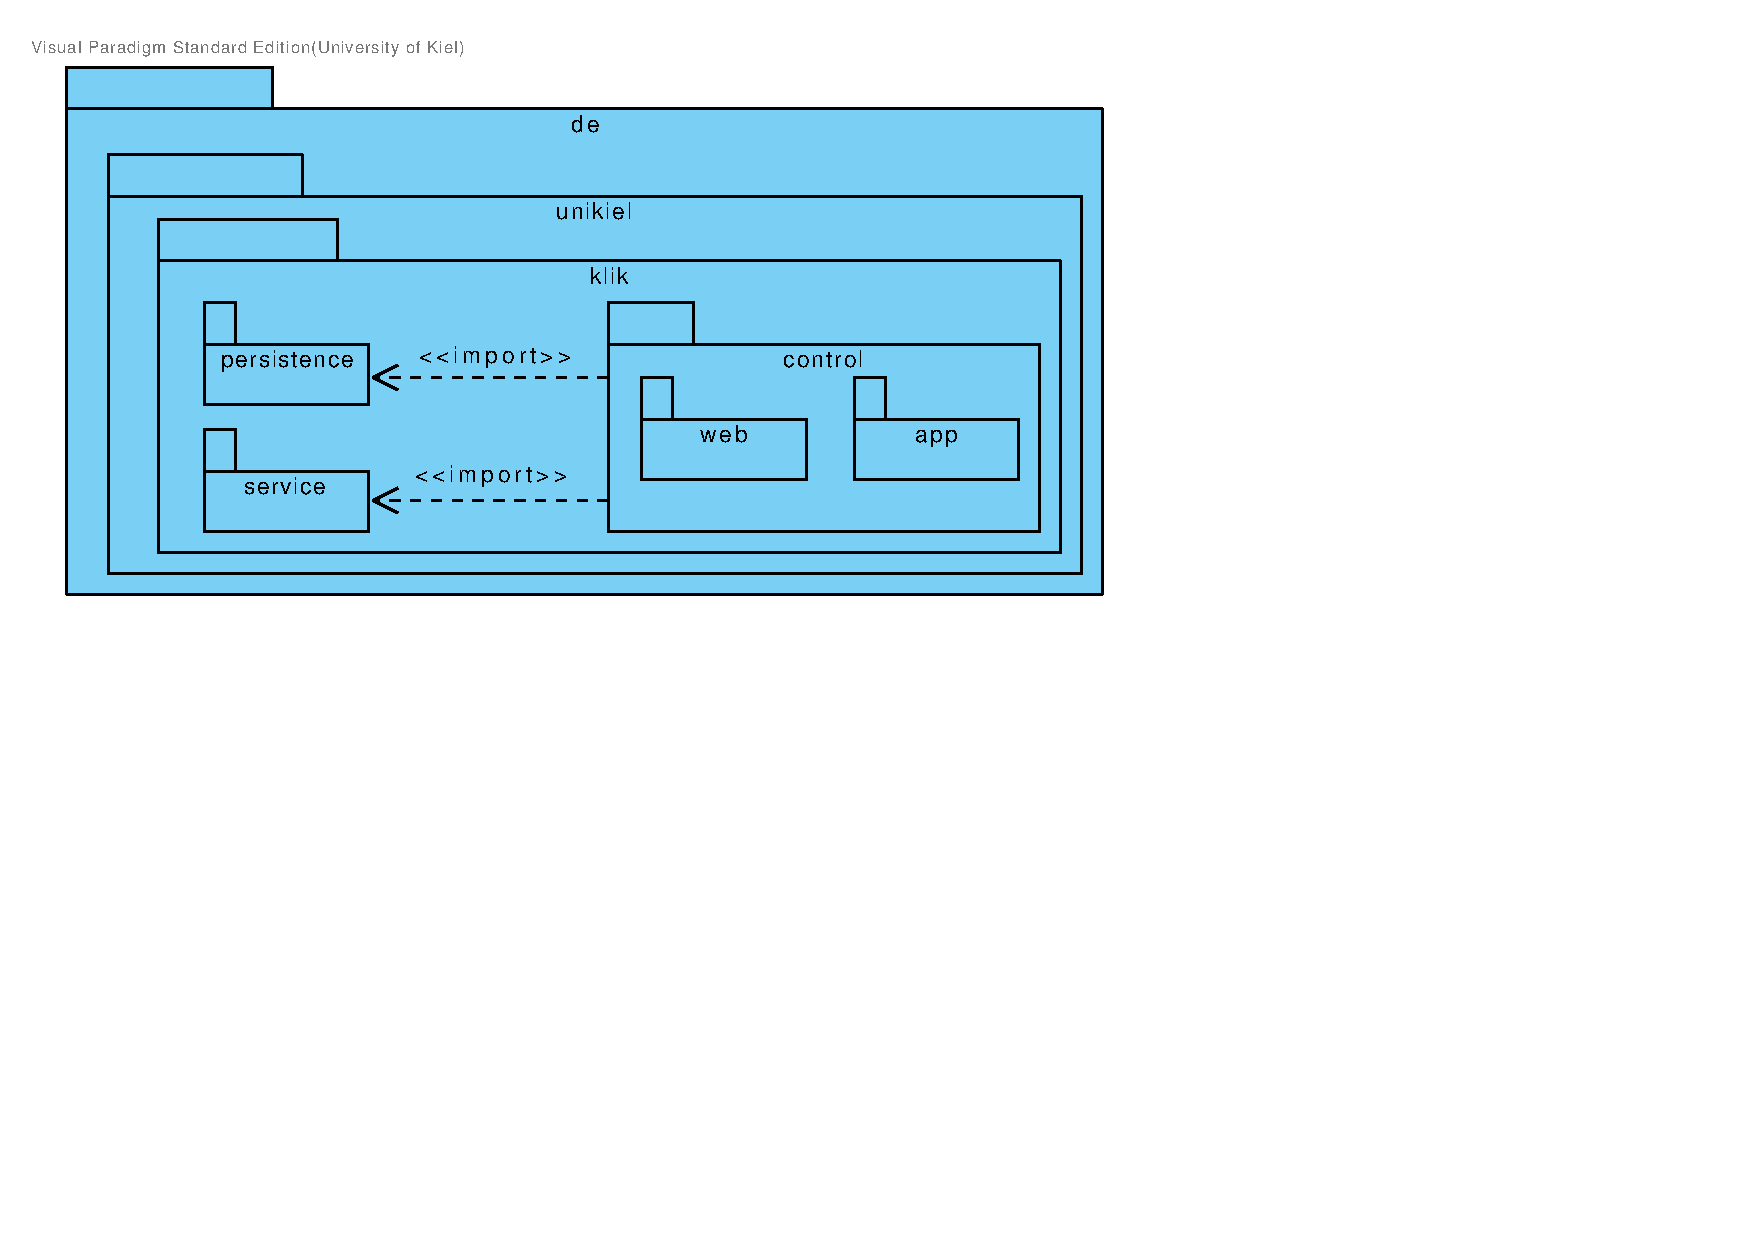
\includegraphics[width=\textwidth, trim=1cm 10cm 11cm 1cm, clip]{gfx/package_diagram}
  \caption{Pakete der Grails Anwendung}
\end{figure}

\paragraph{persistence} In diesem Paket befinden sich die Klassen, die für die Datenhaltung zuständig sind. Das Paket liegt im Grails-Ordner \emph{domain}.
\paragraph{control} In diesem Paket befinden sich die Klassen, die für die Klassen, die Serveranfragen entgegennehmen und diese verarbeiten. Das Paket liegt im Grails-Ordner \emph{controllers}.
\paragraph{control.web} Die Klassen, die Anfragen von der Website entgegen nehmen und diese verarbeiten, befinden sich in diesem Paket.
\paragraph{control.app} Die Klassen, die Anfragen von der Android-App entgegen nehmen und diese verarbeiten, befinden sich in diesem Paket.
\paragraph{service} In diesem Paket befinden sich Klassen, die als Bindeglied zwischen dem \emph{control}- und dem \emph{persistence}-Paket stehen. Dies sind zum einem einen Klassen, die Änderungen auf den Daten vornehmen, und zum anderen Klassen, die Methoden bereitstellen, die von verschiedenen \emph{control}-Klassen verwendet werden. Das Paket liegt im Grails-Ordner \emph{services}.

\subsubsection{Android App}

\begin{figure}[H]
  \centering
  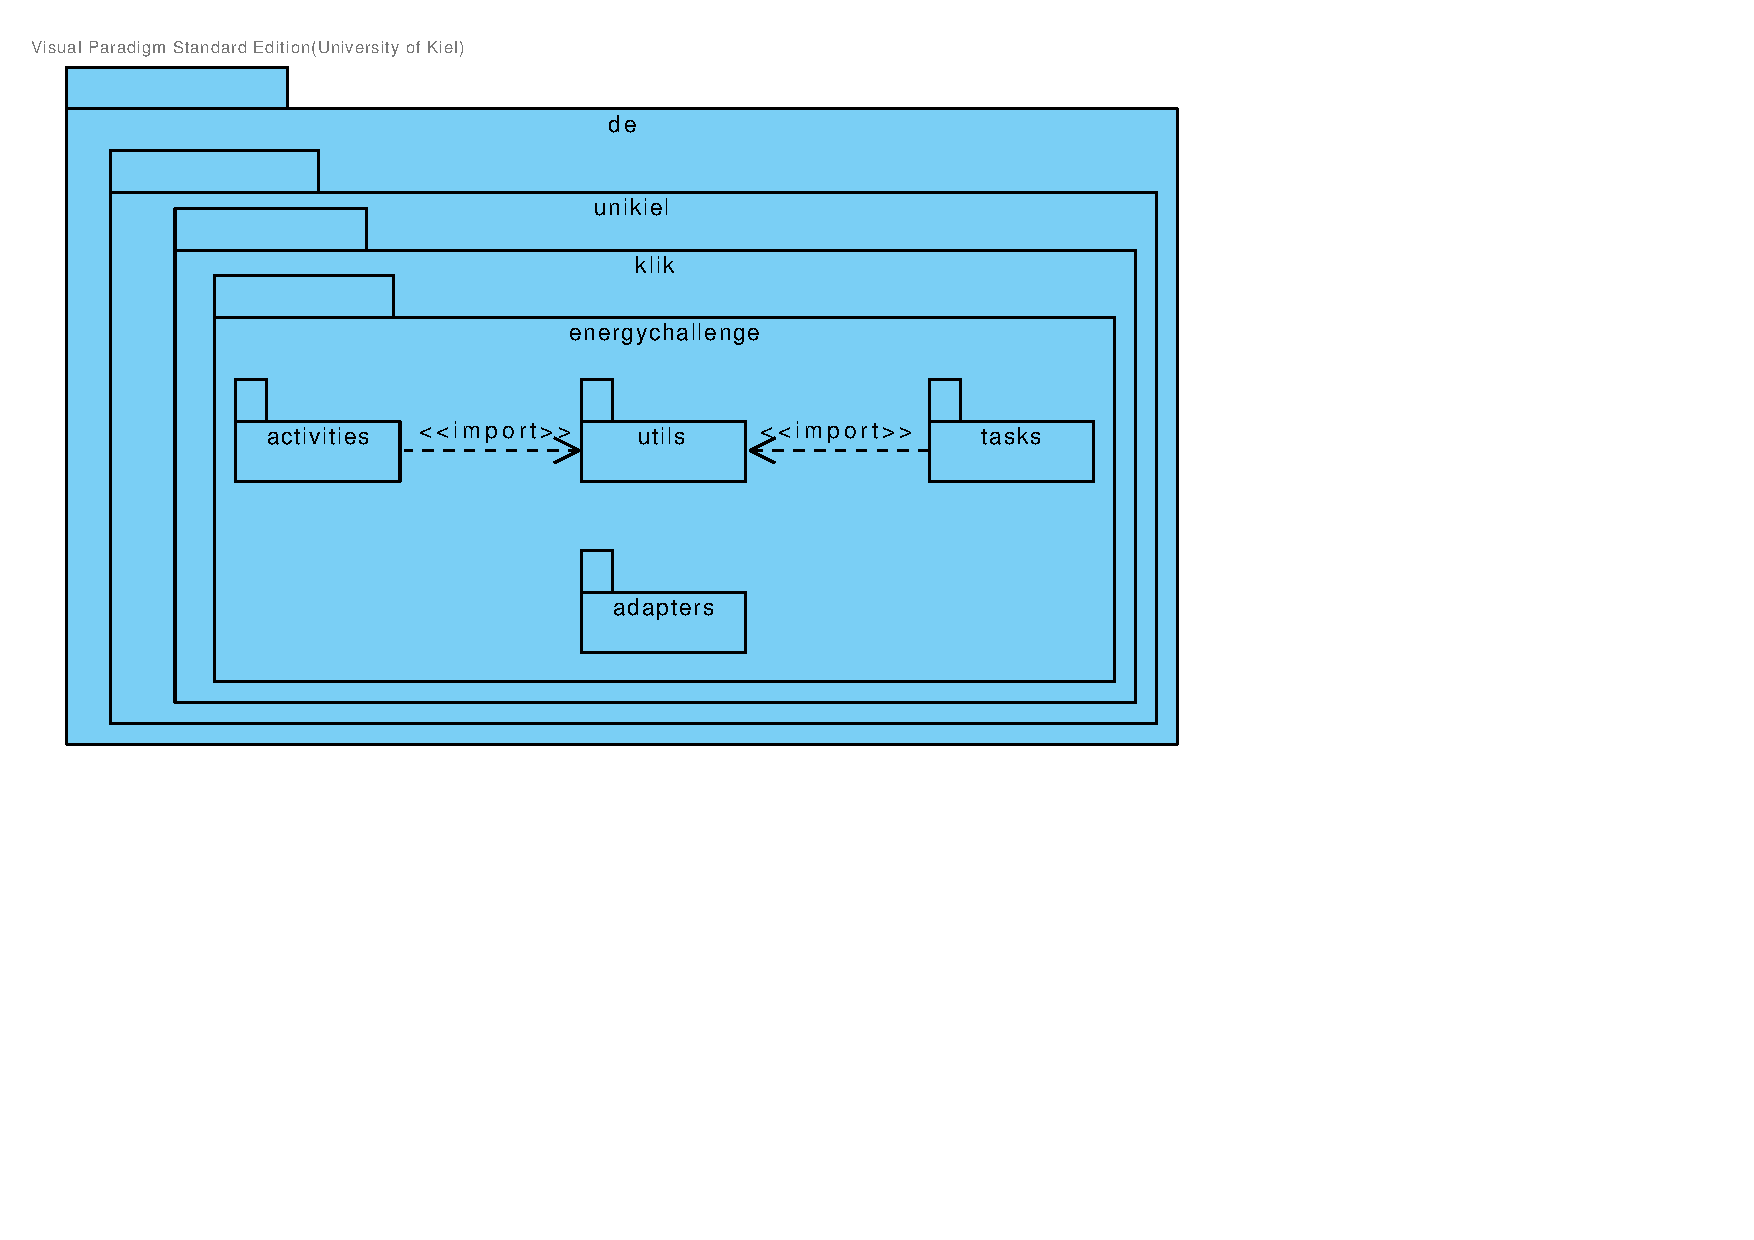
\includegraphics[width=\textwidth, trim=1cm 7cm 9cm 1cm, clip]{gfx/app_package_diagram}
  \caption{Pakete der Android App}
\end{figure}

\paragraph{activties} In diesem Paket befinden sich die Klassen, die die elementaren Bausteine der Android-App sind. Dies sind die \emph{Activity}- und \emph{Fragment}-Klassen. Sie sind für die Anzeige von Inhalten zuständig.
\paragraph{adapters} In diesem Paket befinden sich Klassen, die für die Datenhaltung und Modifizierung der Daten, die in den \emph{Activity}- und \emph{Fragment}-Klassen dargestellt werden, zuständig sind. Dies sind Android-\emph{Adapter}-Klassen.
\paragraph{tasks} In diesem Paket befinden sich Klassen, die für die Kommunikation mit dem Server verwendet werden.
\paragraph{utils} In diesem Paket befinden sich Klassen, die allgemeine Funktionen bereitstellen.
